%\pdfminorversion=4
\documentclass{beamer}
\usepackage{graphicx}
\usepackage{amsfonts}
\usepackage{amsmath,amscd}
\usepackage{chngpage}
\usepackage{tikz}
\usepackage{ifthen}
\usepackage{relsize}
\usepackage{multirow}
\usepackage{cleveref}
\usepackage{url}

\usepackage{ dsfont }


\usetikzlibrary{positioning}
\usetikzlibrary{matrix}
\usetikzlibrary{calc}
\usetikzlibrary{shapes}
\usetikzlibrary{arrows}
\usetikzlibrary{fit}
\usetikzlibrary{decorations}
\usetikzlibrary{snakes}
\usetikzlibrary{shadows}
\pgfdeclarelayer{background}
\pgfdeclarelayer{backbackground}
\pgfdeclarelayer{foreground}
\pgfsetlayers{backbackground,background,main,foreground}


%%%% PICTURE IF CITATION


\usepackage{animate}
\usepackage{color, colortbl}
\usepackage{xspace}
\usepackage{sidecap}

%\usepackage{biblatex}
\usepackage[style=verbose-note]{biblatex}
\bibliography{RNApyro}

\newcommand{\PE}[1]{E(#1)}
\newcommand{\EI}{\text{EI}}
\newcommand{\ES}{\text{ES}}
\newcommand{\ISO}{\text{ISO}}
\newcommand{\Z}[3]{\mathcal{Z}_{\substack{(#1)\\ [#3]}}^{#2}}
\newcommand{\Y}[3]{\mathcal{Y}_{\substack{(#1)\\ [#3]}}^{#2}}
\newcommand{\B}{\mathcal{B}}
\newcommand{\Kron}{\delta}
\newcommand{\ub}{\bullet}
\newcommand{\GCContent}{\texttt{GC}}
\newcommand{\ourprog}{\texttt{IncaRNAtion}}
\newcommand{\RNAinverse}{\texttt{RNAinverse}}

\newcommand{\Ab}{{\sf{A}}}
\newcommand{\Cb}{{\sf{C}}}
\newcommand{\Gb}{{\sf{G}}}
\newcommand{\Ub}{{\sf{U}}}

\newcommand{\SpaceCheating}{\vspace{-0em}}

%\usepackage[numbers]{natbib}
%\usepackage{bibentry}
%
%%Cite in text
%\newcommand{\ignore}[1]{}
%\newcommand{\nobibentry}[1]{{\let\nocite\ignore\bibentry{#1}}}
%% apsrev entries in the text need definitions of these commands
%\newcommand{\bibfnamefont}[1]{#1}
%\newcommand{\bibnamefont}[1]{#1}


%\newcommand{myhighlight}{yellow}
%\usepackage[table]{xcolor}
%\newcolumntype{K}{\columncolor[gray]{0.8}\centering}
% \usepackage{beamerthemesplit} // Activate for custom appearance

\newcommand{\JW}{\href{http://www.cs.mcgill.ca/~jeromew/}{J\'er\^ome Waldisp\"uhl\xspace}}
\newcommand{\YP}{\href{http://www.lix.polytechnique.fr/~ponty/}{Yann Ponty\xspace}}

\newcommand{\lred}[1]{{\Large\textcolor{red}{#1}}}

\setbeamertemplate{frametitle}[default][center]

\usepackage[noend,ruled,vlined]{algorithm2e}


\title{Designing RNA sequences with targeted secondary structure and nucleotide distribution}
\titlegraphic{\includegraphics[width=\textwidth]{Figures/title_fig_2.jpg}}
\author{\underline{Vladimir Reinharz}\\ \YP, \JW\\\textcolor{blue}{vladimir.reinharz@mail.mcgill.ca}}
\date{\today}

\begin{document}

\frame{\titlepage}

\frame{
	\frametitle{RNA Design}
		\begin{figure}
			\centering
				\includegraphics[width=\textwidth]{Figures/logic_gate.png}
			\caption{Rodrigo et al. 2012}
		\end{figure}
			
}

\frame{
	\frametitle{RNA Structure}
	%\lred{FIG 3D -> 2D representation}
	\begin{minipage}{0.4\textwidth}
		\begin{figure}
			\centering
			\includegraphics[height=0.80\textheight,width=\textwidth]{Figures/1LNC.png}
		\end{figure}
	\end{minipage}
	\begin{minipage}{0.5\textwidth}
		\begin{figure}
			\centering
				\includegraphics<2>[width=\textwidth]{Figures/hairpin_stack_0.jpg}
				\includegraphics<3>[width=\textwidth]{Figures/hairpin_stack_1.jpg}
				\includegraphics<4>[width=\textwidth]{Figures/hairpin_stack_2.jpg}
				\includegraphics<5>[width=\textwidth]{Figures/hairpin_stack_3.jpg}
				\includegraphics<6>[width=\textwidth]{Figures/hairpin_stack_4.jpg}
		\end{figure}
	\end{minipage}
}

\frame{
	\frametitle{Affinity Landscape}
		\begin{figure}
			\centering
				\includegraphics<1>[ width=\textwidth]{Figures/energy_1.png}
			%	\includegraphics<2>[ height=0.8\textheight]{Figures/energy_2}
		\end{figure}	
}

\frame{
	\frametitle{Local Design}
	\begin{figure}[tl!]
		\centering
		\includegraphics<1>[width=\textwidth]{Figures/2_hairpins.pdf}
		\includegraphics<2>[width=\textwidth]{Figures/2_hairpins_divided.pdf}
		\includegraphics<3>[width=\textwidth]{Figures/1_hairpin_folding.pdf}
		\includegraphics<4>[width=\textwidth]{Figures/concat_folding.pdf}
	\end{figure}

}

\frame{
	\frametitle{Global Sampling}
	%Since divide and conquer fail, lets look at everything at the same thing
	\begin{itemize}
		\item We can define a Boltzmann distribution
		\item Due to additive properties of the \texttt{Stacking Energy} we can efficiently compute the partition function $\mathds{Z}$ with a 
			Dynamic Programming scheme
	\end{itemize}
	\begin{minipage}{0.45\textwidth}	
		Boltzmann factor:\\ \scalebox{1.5}{$\qquad\mathcal{B}(s):= e^\frac{-\PE{s}}{RT}$}\vspace{7pt}\\
		Partition function:\vspace{7pt}\\\scalebox{1.5}{$\displaystyle\qquad\mathds{Z} = \sum_s\mathcal{B}(s)$}\\\vspace{-15pt}
		\begin{align*}
			\PE{s}:&=\hspace{-20pt}\underbrace{\ES}_{\text{Stacking Energy}}\hspace{-15pt}(s,S)
		\end{align*}	
	\end{minipage}
	\begin{minipage}{0.45\textwidth}
	\begin{figure}
		\centering
		\includegraphics[width=1.2\textwidth]{Figures/boltz_seq.pdf}
	\end{figure}
	\end{minipage}
}

\frame[t]{
	\frametitle{Affinity $\neq$ Specificity}
	\begin{figure}[t]
		\centering
   \only<1>{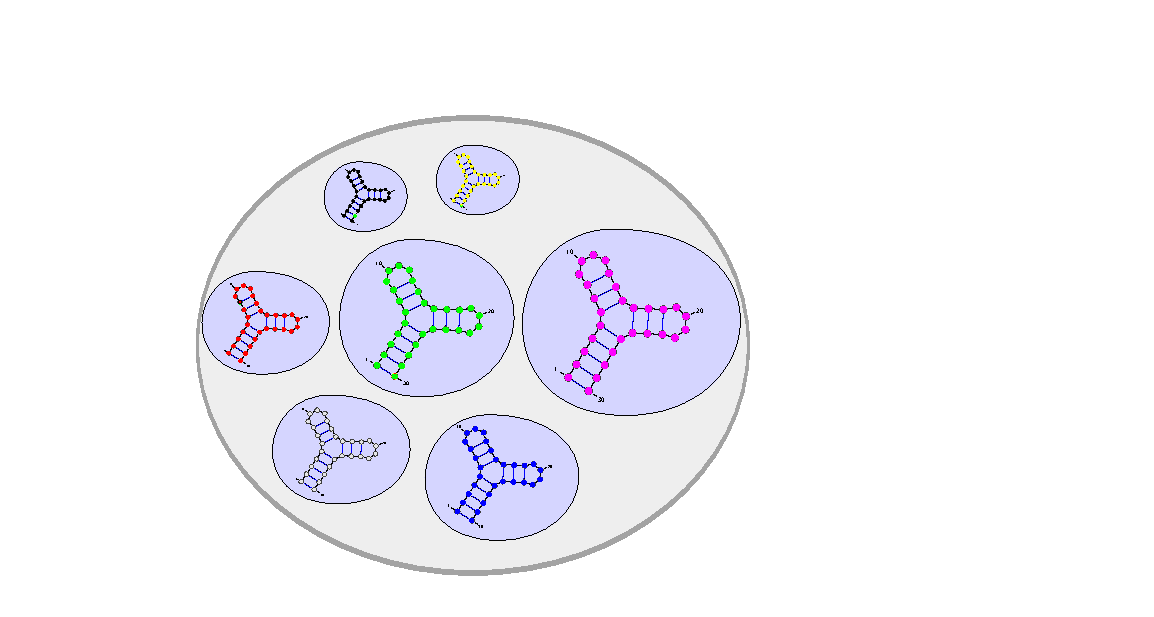
\includegraphics[width=\textwidth]{Figures/boltz_seq_2}}%
   \only<2>{\includegraphics[width=\textwidth]{Figures/boltz_seq_2_a}}%
   \only<3>{\includegraphics[width=\textwidth]{Figures/boltz_seq_2_b}}%
	\end{figure}
  Formally, a large affinity neither {\only<2->{\color{purple}}ensures} preferential fold into a target, 
  {\only<3->{\color{red}}nor is it a necessary condition}\ldots\\
  In practice, viable alternative to local search/genetic algorithms {\relsize{-1}[Levin et al, NAR 2012]}
}


%\frame{
%	\frametitle{Probabilistic Model\\Structure Space}
%	\lred{FIG LARGE SEQUENCE SPACE != LARGE STRUCT SPACE}
%}

\frame{
	\frametitle{\texttt{IncaRNAtion}}
	\begin{table}
	\centering
	\begin{tabular}{cc}
	{\Large \texttt{RNA-ensign\footnote{Levin et al. 2012}}} & {\Large\texttt{IncaRNAtion}}\\\pause
	Seeded & No Seed\\\pause
	Explore mutant space & Explore \textcolor{red}{\textbf{full}} sequence space\\\pause
	$\mathcal{O}(n^5)$ & $\mathcal{O}(n)$\\\pause
	 Complex energy model & Simple energy model\\\pause
	& Sequence constraints
	\end{tabular}
	\end{table}
}

\frame{
	\frametitle{DP Recursion\\global}
	\begin{figure}
		\centering
		\resizebox{0.9\textwidth}{!}{\input{Figures/FigDPInside.pgf}}
	\end{figure}
	Reinharz et al. RECOMB, 2013
}

\frame{
	\frametitle{"Backtrack"\\global}
	\vspace{-5em}
	\begin{figure}
		\centering
		\resizebox{\textwidth}{!}{\input{Figures/FigDPInsideEx.pgf}}
	\end{figure}
}

\frame{
	\frametitle{\texttt{GC} Bias}
%	Energetical bias to high GC content
	\begin{minipage}{0.49\textwidth}
		\begin{figure}
			\centering
			\includegraphics[width=1\textwidth]{Figures/dist_-1.pdf}
	\end{figure}
	\end{minipage}
	\begin{minipage}{0.49\textwidth}
		\begin{figure}
			\centering
			\includegraphics[width=1\textwidth]{Figures/histograme_5_gc_distribution_nornaexinv.png}
		\end{figure}
	\end{minipage}
	
}

\frame{
	\frametitle{Weighted DP Recursion\\global}
	%Change probability to x^{#GC}
	\begin{figure}
		\centering
		\resizebox{\textwidth}{!}{\input{Figures/FigDPInsideWeight.pgf}}
	\end{figure}
}

\frame{
	\frametitle{Incarnation nt distribution\\Bissection scheme}
%	\lred{Cite RECOMB 2012 jerome / yann}
	%Prior distribution kept conditioned by GC to re-enter average around target
	%Once good match, probability to get exactly at target is constant, so search for good value low weight in complexity
	\begin{figure}
		\centering
		\includegraphics<1>[width=0.85\textwidth]{Figures/dist_0.pdf}
		\includegraphics<2>[width=0.85\textwidth]{Figures/dist_1.pdf}
		\includegraphics<3>[width=0.85\textwidth]{Figures/dist_2.pdf}
		\includegraphics<4>[width=0.85\textwidth]{Figures/dist_3.pdf}
		\includegraphics<5>[width=0.85\textwidth]{Figures/dist_4.pdf}
	\end{figure}
	 Waldisp\"uhl and Y. Ponty, 2012
}

\frame{
	\frametitle{Incarnation + RNAinverse Results\\Sequence identity}
%	\lred{Only keep length?}
	\begin{figure}[rt]
		\centering
		\includegraphics[width=1.1\textwidth]{Figures/identity_2.pdf}
	\end{figure}
}

\frame{
	\frametitle{Incarnation + RNAinverse time}
	\begin{figure}[t!]
		\centering
		\includegraphics[width=0.9\textwidth]{Figures/time.pdf}
	\end{figure}
}

\frame{
	\frametitle{Future}
	\begin{itemize}
		\item Full energy model
		\item Include other seeded methods
		\item Convince people to make the molecules in labs
	\end{itemize}
}

\frame{
	\frametitle{Acknowledgments}
	\begin{minipage}{0.45\textwidth}
		\begin{itemize}
			\item Coauthors
			\begin{itemize}
				\item \JW
				\item \YP		
			\end{itemize}
		\end{itemize}	
		\begin{figure}
			\centering
			\includegraphics[width=0.5\textwidth]{Figures/logofsm}
		\end{figure}
		\begin{itemize}
			\item Erasmus TEE  fellowship
			\item Travel funding to ISMB/ECCB 2013 was generously provided by ISCB.
		\end{itemize}
	\end{minipage}
	\begin{minipage}{0.45\textwidth}
		\begin{minipage}{0.45\textwidth}
		\begin{figure}
			\centering
			\includegraphics[width=\textwidth]{Figures/logosysbio}
		\end{figure}
		\begin{figure}
			\centering
			\includegraphics[width=\textwidth]{Figures/logoanr.png}
		\end{figure}
		\begin{figure}
				\centering
			\includegraphics[width=\textwidth]{Figures/logoinria.png}
		\end{figure}
		\begin{figure}
			\centering
			\includegraphics[width=\textwidth]{Figures/logofqrnt.png}
		\end{figure}
		\end{minipage}
		\begin{minipage}{0.45\textwidth}
		\begin{figure}
			\centering
			\includegraphics[width=\textwidth]{Figures/logonserc}
		\end{figure}
		\begin{figure}
			\centering
			\includegraphics[width=\textwidth]{Figures/logocnrs}
		\end{figure}
		\begin{figure}
			\centering
			\includegraphics[width=\textwidth]{Figures/logo_X}
		\end{figure}
		\begin{figure}
			\centering
			\includegraphics[width=0.5\textwidth]{Figures/logolri}
		\end{figure}
		\end{minipage}
	\end{minipage}
}

\frame{
	\frametitle{Success Rate}
	\begin{figure}
		\centering
		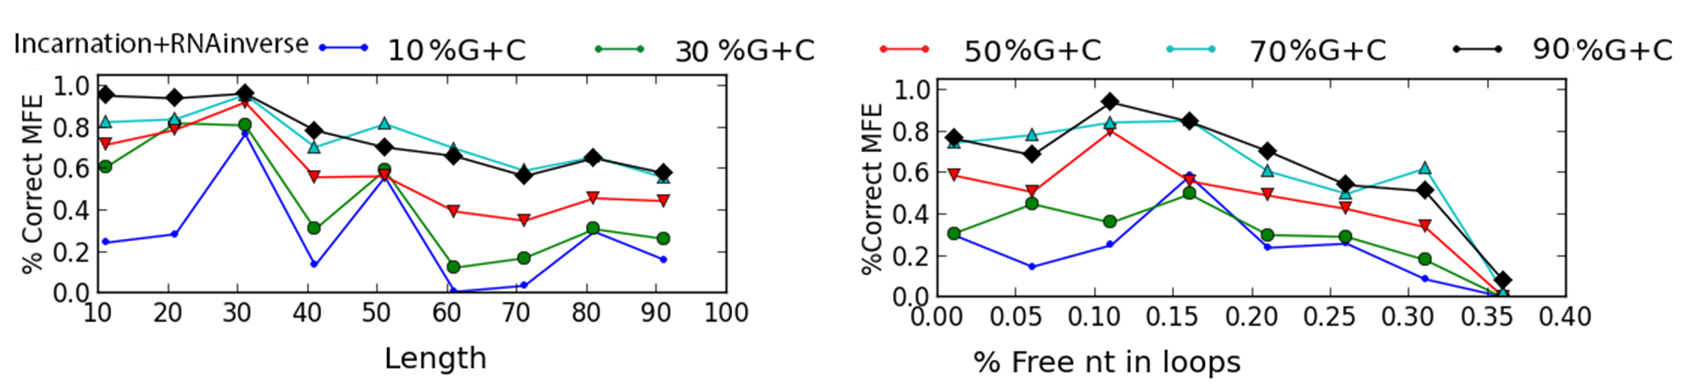
\includegraphics[width=\textwidth]{Figures/results_incar_rnainverse}
	\end{figure}
}

\frame{
	\frametitle{Sensitivity}
	\begin{figure}
		\centering
		\includegraphics[width=\textwidth]{Figures/Sensitivity}
	\end{figure}
}

%
%\frame{
%	\frametitle{And so...}
%		\begin{itemize}
%			\item It kinda works
%			\item Energetic model really simple
%			\item Exploit sequences with wanted structures (but wrong GC content).
%		\end{itemize}
%	\begin{minipage}{0.45\textwidth}
%		\begin{equation*}
%		\label{eq:Z_rec}
%		\resizebox{\textwidth}{!}{%
%			$\Z{i,j}{m}{a,b}:=\left\{
%	  \begin{array}{ll}
%  		\displaystyle
%      \sum_{\substack{a'\in \B,\\ \Kron_{a',s_i}\le m}}  
%      \Z{i+1,j}{m-\Kron_{a',s_i}}{a',b} & \text{If }S_{i}=-1\\
%      \displaystyle
%      \sum_{\substack{a',b'\in \B^2,\\ \Kron_{a'b',s_is_j}\le m}}
%			 e^{\frac{-E_{(i,j),ab \to a'b'}^{\Omega,\beta}}{RT}}
%			 \cdot \Z{i+1,j-1}{m-\Kron_{a'b',s_is_j}}{a',b'}&
%			 \text{Elif }S_i=j \land S_{i-1}=j+1\\
%			 \displaystyle
%      \sum_{\substack{a',b'\in \B^2,\\ \Kron_{a'b',s_is_k}\le m}}
%      \sum_{m'=0}^{m-\Kron_{a'b',s_is_k}}
%   		 e^{\frac{-E_{(i,k),\varnothing\to a'b'}^{\Omega,\beta}}{RT}}
%      \cdot\Z{i+1,k-1}{m-\Kron_{a'b',s_is_k}-m'}{a',b'}
%      \cdot\Z{k+1,j}{m'}{b',b} & \text{Elif }S_i=k \land i < k \leq j\\
%      0 &\text{Otherwise}
%		\end{array}\right.$}
%		\end{equation*}
%	\end{minipage}
%	\begin{minipage}{0.45\textwidth}
%	\begin{algorithm}[t]
%		\DontPrintSemicolon
%		\SetAlgoLined
%		\SetKwFunction{Backtrack}{SB$_x$}
%		\SetKwFunction{Random}{Random}
%		\newcommand{\rand}{{r}}
%		$\rand \leftarrow $\Random$\left(\Z{\N,\Struct}{a,b}\right)$\tcp*[r]{Random 		real in $[0,\Z{\N,\Struct}{a,b}[$}
%		 \Switch{}{
%   		\lCase(\tcp*[f]{Empty structure}){$\Struct=\varepsilon$}{\Return{$\varepsilon$}}
%		  \Case(\tcp*[f]{First position is unpaired}){$\Struct=\ub\, \Struct'$}{		
%   			\For{$a'\in\B$}{
%					$\rand \leftarrow \rand - x^{\gc(a')}\cdot \Z{\BoolFalse,\Struct'}{a',b}$\;
%					\lIf{$\rand<0$}\Return{$a'.\Backtrack(a',b,\BoolFalse,\Struct')$}\;
%  			}
%   		}
%	   	\Case(\tcp*[f]{Extremities are involved in stacking base pair}){$\Struct=			\text{\rm\op}\, \Struct' \,\text{\rm\cp}$  {\rm \bf and} $\N=\BoolTrue$}
%   		{		
%				\For{$(a',b')\in\B\times\B$}
%    		{
%					$\rand \leftarrow \rand -
%			 		x^{\gc(a'.b')}
%			 		\cdot e^{{-\ES^{\beta}_{ab \to a'b'}}/{RT}}
%			 		\cdot \Z{\BoolTrue,\Struct'}{a',b'}	$\;
%					\lIf{$\rand<0$}{
%						\Return{$a'.\Backtrack(a',b',\BoolTrue,\Struct'). b'$}\;		
%					}
%				}
%			}
%   		\Other(\tcp*[f]{First position is paired without a stacking pair})
%   		{
%				\tcp{$\Struct=\text{\rm\op}\, \Struct' \,\text{\rm\cp}\,\Struct''$}
%				\For{$(a',b')\in\B\times\B$}{
%					$\rand \leftarrow \rand -	
%    	   	x^{\gc(a'.b')}
%					\cdot e^{\frac{-\ES^{\beta}_{\varnothing\to a'b'}}{RT}}
%	  	    \cdot\Z{\BoolFalse,\Struct'}{a',b'}
%	      	\cdot\Z{\BoolTrue,\Struct''}{b',b}$\;	
% 					\lIf{\rand $<0$}{
%						\Return{$a'
%							.\Backtrack\left(a',b',\BoolTrue,\Struct'\right)
%							.b'
%							.\Backtrack\left(b',b,\BoolFalse,\Struct''\right)
%						$}\;	
%					}
%				}
%   		}
%	 	}
%%\caption{\protect\Backtrack$\left(a,b,\N,\Struct\right)$\label{alg:back}}
%\end{algorithm}
%\end{minipage}
%}


%\frame{
%	\frametitle{RNA Design}
%	{\Large Logic gates!
%	}
%	\begin{figure}
%		\centering
%		\includegraphics[width=\textwidth]{Figures/and_gate.jpg}
%	\end{figure}
%}
%
%
%\frame{
%	\frametitle{RNA Structure}
%	\begin{minipage}{0.45\textwidth}
%		\begin{figure}
%			\centering
%			\includegraphics[height=0.7\textheight]{Figures/riboswitch_rna.jpg}
%		\end{figure}
%	\end{minipage}
%	\begin{minipage}{0.45\textwidth}
%		\begin{figure}
%			\centering
%			\includegraphics[angle=90,height=0.8\textheight]{Figures/varna_2d.eps}
%		\end{figure}
%	\end{minipage}
%}
%
%\frame{
%	\frametitle{Base pairs}
%	\begin{figure}[ht]
%		\centering
%		\includegraphics[height=0.7\textheight]{Figures/canonical_bps.png}
%	\end{figure}
%
%}
%
%
%\frame{
%	\frametitle{Algorithmic}
%	\begin{itemize}\Large
%	\item Secondary structure prediction is \textbf{"easy"}
%	\item Sequence design is \textbf{hard}
%	\end{itemize}•
%}
%
%
%
%
%\frame{
%	\frametitle{Simple Pseudo-Energy\\Additive Stacking-Pairs}
%		\begin{itemize}
%			\item Experimentally determined for every stacked canonical base pairs  						between $-3.5$ and $+1$
%			\item Know for stacks of \{\texttt{AU,GC,GU}\}, else parameter $\beta$ which can be $+\infty$ 					
%		\end{itemize}	
%		\begin{figure}
%				\centering
%					\includegraphics<1>[width=0.6\textwidth]{Figures/hairpin_stack_0.jpg}
%					\includegraphics<2>[width=0.6\textwidth]{Figures/hairpin_stack_1.jpg}
%					\includegraphics<3>[width=0.6\textwidth]{Figures/hairpin_stack_2.jpg}
%					\includegraphics<4>[width=0.6\textwidth]{Figures/hairpin_stack_3.jpg}
%					\includegraphics<5>[width=0.6\textwidth]{Figures/hairpin_stack_4.jpg}
%			\end{figure}
%}
%
%\frame{
%	\frametitle{Base pairs}
%	\begin{figure}[ht]
%		\centering
%		\includegraphics[height=0.7\textheight]{Figures/canonical_bps.png}
%	\end{figure}
%
%}
%
%
%\frame{
%	\frametitle{Local Design (roughly)}
%	\begin{itemize}
%		\item Cut structure in pieces
%		\item Find sub-sequences folding into pieces
%		\item Concatenate them, pray
%	\end{itemize}
%}	
%
%\frame{
%	\frametitle{Pseudo RNAinverse method\\local}
%	\vspace{-5em}
%	\begin{figure}
%		\centering
%		\resizebox{\textwidth}{!}{%!TEX root = ../axearn.tex
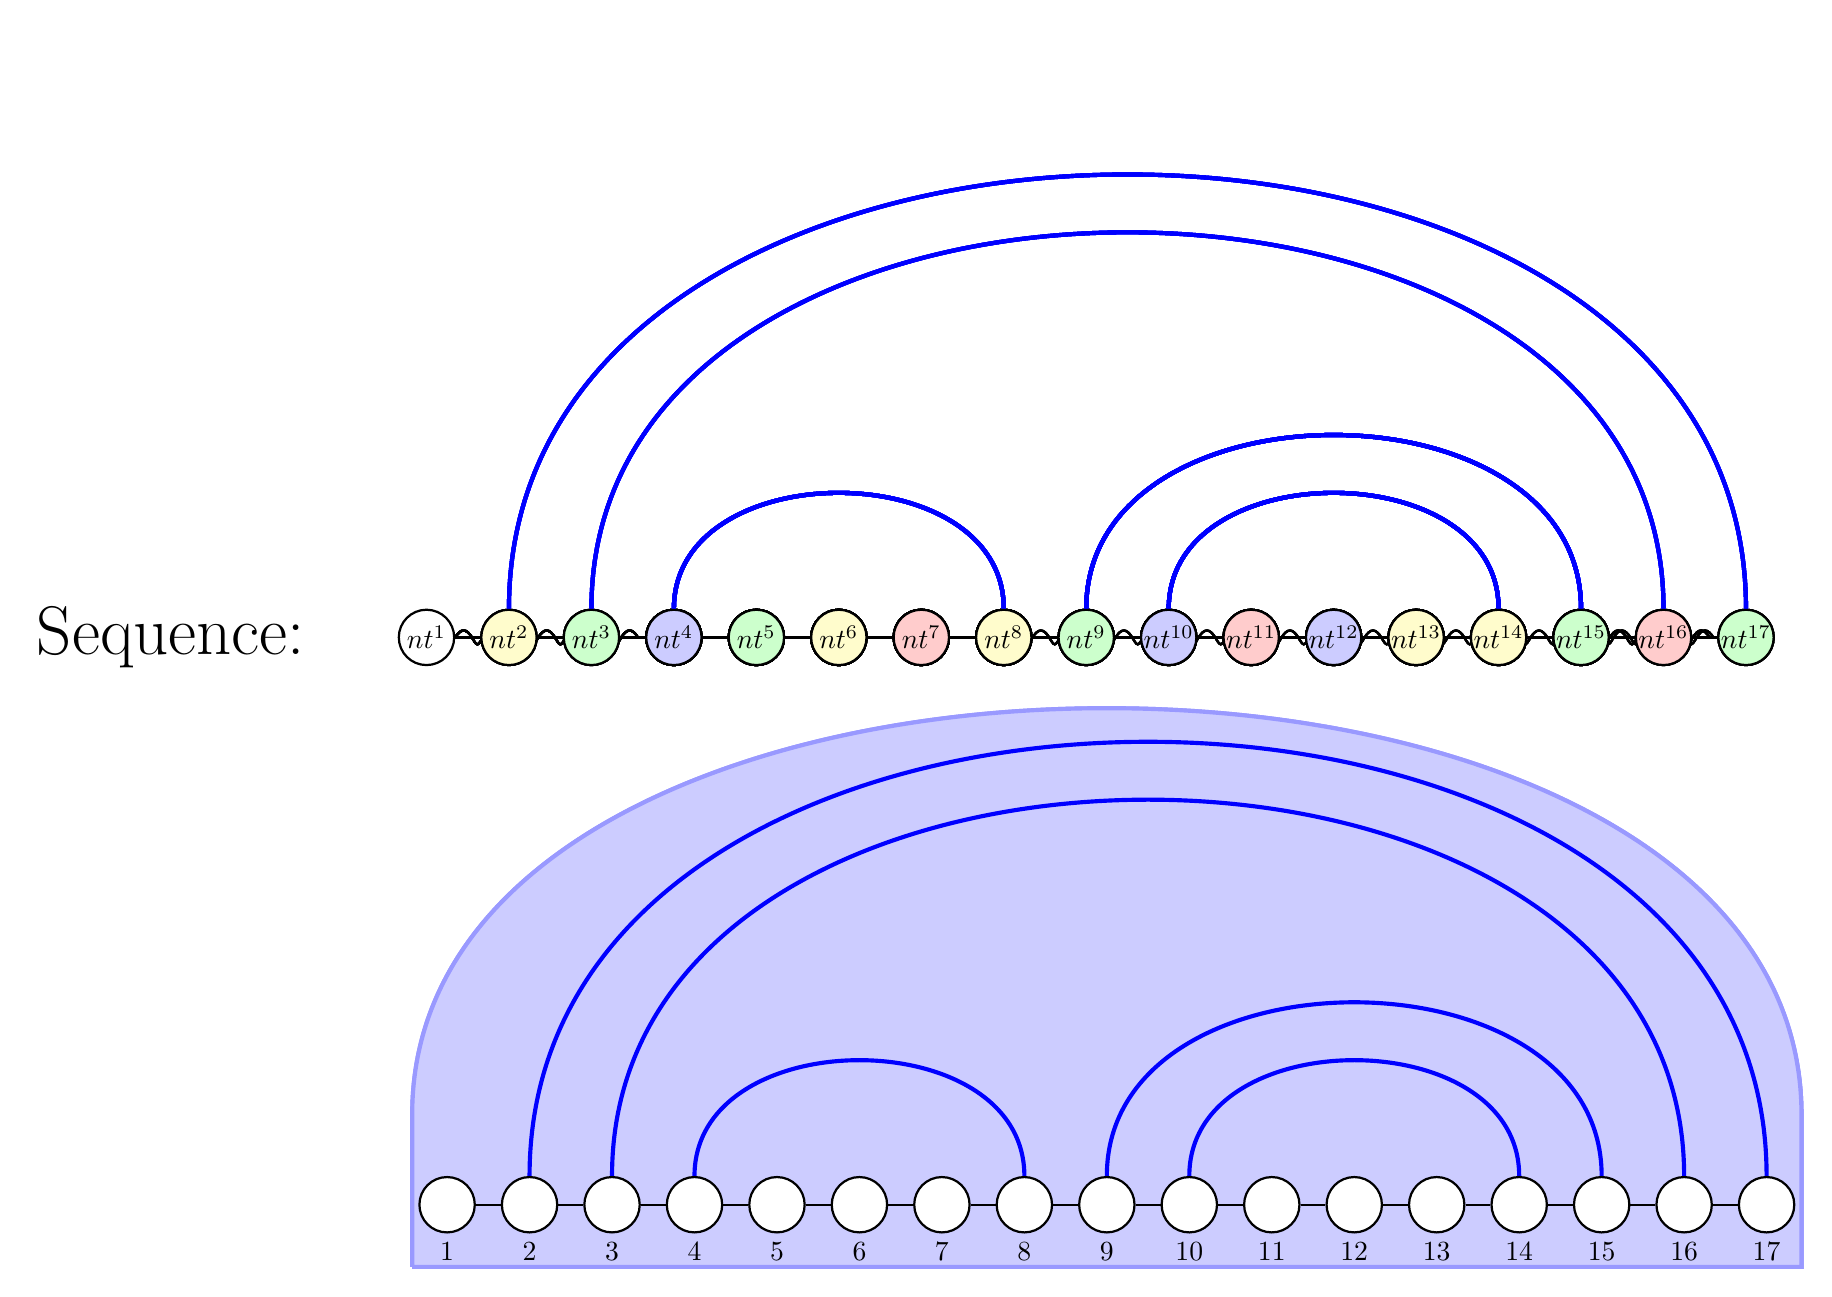
\begin{tikzpicture}

 \newcommand{\BSep}{9pt}
 \newcommand{\ESep}{30pt}
 \newcommand{\HSep}{250pt}
  \tikzstyle{base}=[circle,draw,thick,inner sep=0,minimum width=20pt,fill=white]
%  \tikzstyle{basered}=[circle,draw,thick,inner sep=0,minimum width=20pt,fill=red]
  \tikzstyle{basesmall}=[circle,draw,thick,inner sep=0,minimum width=10pt,fill=white]
  \tikzstyle{basephantom}=[base,dashed]
    \tikzstyle{baseinvisible}=[base,dashed,opacity=0]
  \tikzstyle{linez}=[draw,snake=coil, segment aspect=.2,%
line after snake=0pt, 
        segment length=10pt,thick]
  \tikzstyle{lined}=[linez,draw,snake=none,thick]
  \tikzstyle{line}=[linez,draw,snake=none,thick]
  \tikzstyle{bp}=[in=90,out=90,draw,line width=1.5pt,blue,looseness=1.2]
  \tikzstyle{bptransparent}=[in=90,out=90,draw,line width=1.5pt,blue!20,looseness=1.2]  
  \tikzstyle{redbp}=[in=90,out=90,draw,line width=1.5pt,red,looseness=1.2]
  \tikzstyle{inblock}=[trapezium,trapezium angle=83, fill=blue!20, draw=blue!40,line width=1.5pt, inner sep=0]
    \tikzstyle{inblockgray}=[trapezium,trapezium angle=83, fill=lightgray!20, draw=lightgray,line width=1.5pt, inner sep=0]
   \tikzstyle{outblock}=[trapezium,trapezium angle=83, fill=red!50, draw=red!40,line width=1.5pt, inner sep=0]
  \tikzstyle{lbl}=[inner sep=0]
  \tikzstyle{arr}=[line width=1.3pt,->]
%

\begin{scope}[yshift=185pt]
  \node[] (tot) at (0,0) {\Huge Sequence:};
	\visible<2-2>{
		\node[right=\ESep of tot, baseinvisible] (iso-a-1) {$nt^1$};
		\foreach \i in {2,...,17}{
			\pgfmathtruncatemacro\j{\i - 1}
			\ifthenelse{\i>3 \and \i<9}{
					\node[right=\BSep of iso-a-\j, base] (iso-a-\i) {$nt^{\i}$};		
					\ifthenelse{\i>4}
						{\path[lined] (iso-a-\j) -- (iso-a-\i);}
						{}
				}{
					\node[right=\BSep of iso-a-\j, baseinvisible] (iso-a-\i) {$nt^{\i}$};
				}
		}
			\path[linez] (iso-a-1) to (iso-a-4);
			\path[linez] (iso-a-8) to (iso-a-17);
			\draw[bp] (iso-a-4) to (iso-a-8);
	}
	
	\visible<3>{
		\node[right=\ESep of tot, baseinvisible] (iso-a-1) {$nt^1$};
		\foreach \i in {2,...,17}{
			\pgfmathtruncatemacro\j{\i - 1}
			\ifthenelse{\i>3 \and \i<9}{
				\ifthenelse{\i=4}{\node[right=\BSep of iso-a-\j, base,fill=blue] (iso-a-\i) {$nt^{\i}$};}{				        
				\ifthenelse{\i=5}{\node[right=\BSep of iso-a-\j, base,fill=green] (iso-a-\i) {$nt^{\i}$};}{
				\ifthenelse{\i=6}{\node[right=\BSep of iso-a-\j, base,fill=yellow] (iso-a-\i) {$nt^{\i}$};}{
				\ifthenelse{\i=7}{\node[right=\BSep of iso-a-\j, base,fill=blue] (iso-a-\i) {$nt^{\i}$};}{
				\ifthenelse{\i=8}{\node[right=\BSep of iso-a-\j, base,fill=red] (iso-a-\i) {$nt^{\i}$};}{
				}}}}}
				\ifthenelse{\i>4}
					{\path[lined] (iso-a-\j) -- (iso-a-\i);}
					{}
			}{
				\node[right=\BSep of iso-a-\j, baseinvisible] (iso-a-\i) {$nt^{\i}$};
			}
		}
			\path[linez] (iso-a-1) to (iso-a-4);
			\path[linez] (iso-a-8) to (iso-a-17);
			\draw[bp] (iso-a-4) to (iso-a-8);
	}
	
	\visible<4>{
		\node[right=\ESep of tot, baseinvisible] (iso-a-1) {$nt^1$};
		\foreach \i in {2,...,17}{
			\pgfmathtruncatemacro\j{\i - 1}
			\ifthenelse{\i>3 \and \i<9}{
				\ifthenelse{\i=4}{\node[right=\BSep of iso-a-\j, base,fill=blue] (iso-a-\i) {$nt^{\i}$};}{				        
				\ifthenelse{\i=5}{\node[right=\BSep of iso-a-\j, base,fill=green!20] (iso-a-\i) {$nt^{\i}$};}{
				\ifthenelse{\i=6}{\node[right=\BSep of iso-a-\j, base,fill=yellow!20] (iso-a-\i) {$nt^{\i}$};}{
				\ifthenelse{\i=7}{\node[right=\BSep of iso-a-\j, base,fill=blue!20] (iso-a-\i) {$nt^{\i}$};}{
				\ifthenelse{\i=8}{\node[right=\BSep of iso-a-\j, base,fill=red] (iso-a-\i) {$nt^{\i}$};}{
				}}}}}
				\ifthenelse{\i>4}
					{\path[lined] (iso-a-\j) -- (iso-a-\i);}
					{}
			}{
				\node[right=\BSep of iso-a-\j, baseinvisible] (iso-a-\i) {$nt^{\i}$};
			}
		}
			\path[linez] (iso-a-1) to (iso-a-4);
			\path[linez] (iso-a-8) to (iso-a-17);
			\draw[bp] (iso-a-4) to (iso-a-8);
	}
	
	\visible<5>{
		\node[right=\ESep of tot, baseinvisible] (iso-a-1) {$nt^1$};
		\foreach \i in {2,...,17}{
			\pgfmathtruncatemacro\j{\i - 1}
			\ifthenelse{\i>3 \and \i<9}{
				\ifthenelse{\i=4}{\node[right=\BSep of iso-a-\j, base,fill=green] (iso-a-\i) {$nt^{\i}$};}{				        
				\ifthenelse{\i=5}{\node[right=\BSep of iso-a-\j, base,fill=green!20] (iso-a-\i) {$nt^{\i}$};}{
				\ifthenelse{\i=6}{\node[right=\BSep of iso-a-\j, base,fill=yellow!20] (iso-a-\i) {$nt^{\i}$};}{
				\ifthenelse{\i=7}{\node[right=\BSep of iso-a-\j, base,fill=blue!20] (iso-a-\i) {$nt^{\i}$};}{
				\ifthenelse{\i=8}{\node[right=\BSep of iso-a-\j, base,fill=yellow] (iso-a-\i) {$nt^{\i}$};}{
				}}}}}
				\ifthenelse{\i>4}
					{\path[lined] (iso-a-\j) -- (iso-a-\i);}
					{}
			}{
				\node[right=\BSep of iso-a-\j, baseinvisible] (iso-a-\i) {$nt^{\i}$};
			}
		}
			\path[linez] (iso-a-1) to (iso-a-4);
			\path[linez] (iso-a-8) to (iso-a-17);
			\draw[bp] (iso-a-4) to (iso-a-8);
	}
	
	\visible<6>{
		\node[right=\ESep of tot, baseinvisible] (iso-a-1) {$nt^1$};
		\foreach \i in {2,...,17}{
			\pgfmathtruncatemacro\j{\i - 1}
			\ifthenelse{\i>3 \and \i<16}{
				\ifthenelse{\i=4}{\node[right=\BSep of iso-a-\j, base,fill=green!20] (iso-a-\i) {$nt^{\i}$};}{
				\ifthenelse{\i=5}{\node[right=\BSep of iso-a-\j, base,fill=green!20] (iso-a-\i) {$nt^{\i}$};}{
				\ifthenelse{\i=6}{\node[right=\BSep of iso-a-\j, base,fill=yellow!20] (iso-a-\i) {$nt^{\i}$};}{
				\ifthenelse{\i=7}{\node[right=\BSep of iso-a-\j, base,fill=blue!20] (iso-a-\i) {$nt^{\i}$};}{
				\ifthenelse{\i=8}{\node[right=\BSep of iso-a-\j, base,fill=yellow!20] (iso-a-\i) {$nt^{\i}$};}{
				\node[right=\BSep of iso-a-\j, base] (iso-a-\i) {$nt^{\i}$};
				}}}}}
				\ifthenelse{\i>4}
					{\path[lined] (iso-a-\j) -- (iso-a-\i);}
					{}
			}{
				\node[right=\BSep of iso-a-\j, baseinvisible] (iso-a-\i) {$nt^{\i}$};
			}
		}
			\path[linez] (iso-a-1) to (iso-a-4);
			\path[linez] (iso-a-15) to (iso-a-17);
			\draw[bptransparent] (iso-a-4) to (iso-a-8);
			\draw[bp] (iso-a-9) to (iso-a-15);
			\draw[bp] (iso-a-10) to (iso-a-14);
	}
	
	\visible<7>{
		\node[right=\ESep of tot, baseinvisible] (iso-a-1) {$nt^1$};
		\foreach \i in {2,...,17}{
			\pgfmathtruncatemacro\j{\i - 1}
			\ifthenelse{\i>3 \and \i<16}{
				\ifthenelse{\i=4}{\node[right=\BSep of iso-a-\j, base,fill=green!20] (iso-a-\i) {$nt^{\i}$};}{
				\ifthenelse{\i=5}{\node[right=\BSep of iso-a-\j, base,fill=green!20] (iso-a-\i) {$nt^{\i}$};}{
				\ifthenelse{\i=6}{\node[right=\BSep of iso-a-\j, base,fill=yellow!20] (iso-a-\i) {$nt^{\i}$};}{
				\ifthenelse{\i=7}{\node[right=\BSep of iso-a-\j, base,fill=blue!20] (iso-a-\i) {$nt^{\i}$};}{
				\ifthenelse{\i=8}{\node[right=\BSep of iso-a-\j, base,fill=yellow!20] (iso-a-\i) {$nt^{\i}$};}{
				\ifthenelse{\i=9}{\node[right=\BSep of iso-a-\j, base,fill=yellow] (iso-a-\i) {$nt^{\i}$};}{
				\ifthenelse{\i=10}{\node[right=\BSep of iso-a-\j, base,fill=red] (iso-a-\i) {$nt^{\i}$};}{
				\ifthenelse{\i=11}{\node[right=\BSep of iso-a-\j, base,fill=red] (iso-a-\i) {$nt^{\i}$};}{
				\ifthenelse{\i=12}{\node[right=\BSep of iso-a-\j, base,fill=blue] (iso-a-\i) {$nt^{\i}$};}{
				\ifthenelse{\i=13}{\node[right=\BSep of iso-a-\j, base,fill=yellow] (iso-a-\i) {$nt^{\i}$};}{
				\ifthenelse{\i=14}{\node[right=\BSep of iso-a-\j, base,fill=green] (iso-a-\i) {$nt^{\i}$};}{
				\ifthenelse{\i=15}{\node[right=\BSep of iso-a-\j, base,fill=green] (iso-a-\i) {$nt^{\i}$};}{
				}}}}}}}}}}}}
				\ifthenelse{\i>4}
					{\path[lined] (iso-a-\j) -- (iso-a-\i);}
					{}
			}{
				\node[right=\BSep of iso-a-\j, baseinvisible] (iso-a-\i) {$nt^{\i}$};
			}
		}
			\path[linez] (iso-a-1) to (iso-a-4);
			\path[linez] (iso-a-15) to (iso-a-17);
			\draw[bptransparent] (iso-a-4) to (iso-a-8);
			\draw[bp] (iso-a-9) to (iso-a-15);
			\draw[bp] (iso-a-10) to (iso-a-14);
	}
	
	\visible<8>{
		\node[right=\ESep of tot, baseinvisible] (iso-a-1) {$nt^1$};
		\foreach \i in {2,...,17}{
			\pgfmathtruncatemacro\j{\i - 1}
			\ifthenelse{\i>3 \and \i<16}{
				\ifthenelse{\i=4}{\node[right=\BSep of iso-a-\j, base,fill=green!20] (iso-a-\i) {$nt^{\i}$};}{
				\ifthenelse{\i=5}{\node[right=\BSep of iso-a-\j, base,fill=green!20] (iso-a-\i) {$nt^{\i}$};}{
				\ifthenelse{\i=6}{\node[right=\BSep of iso-a-\j, base,fill=yellow!20] (iso-a-\i) {$nt^{\i}$};}{
				\ifthenelse{\i=7}{\node[right=\BSep of iso-a-\j, base,fill=blue!20] (iso-a-\i) {$nt^{\i}$};}{
				\ifthenelse{\i=8}{\node[right=\BSep of iso-a-\j, base,fill=yellow!20] (iso-a-\i) {$nt^{\i}$};}{
				\ifthenelse{\i=9}{\node[right=\BSep of iso-a-\j, base,fill=red] (iso-a-\i) {$nt^{\i}$};}{
				\ifthenelse{\i=10}{\node[right=\BSep of iso-a-\j, base,fill=red!20] (iso-a-\i) {$nt^{\i}$};}{
				\ifthenelse{\i=11}{\node[right=\BSep of iso-a-\j, base,fill=red!20] (iso-a-\i) {$nt^{\i}$};}{
				\ifthenelse{\i=12}{\node[right=\BSep of iso-a-\j, base,fill=blue!20] (iso-a-\i) {$nt^{\i}$};}{
				\ifthenelse{\i=13}{\node[right=\BSep of iso-a-\j, base,fill=yellow!20] (iso-a-\i) {$nt^{\i}$};}{
				\ifthenelse{\i=14}{\node[right=\BSep of iso-a-\j, base,fill=green!20] (iso-a-\i) {$nt^{\i}$};}{
				\ifthenelse{\i=15}{\node[right=\BSep of iso-a-\j, base,fill=blue] (iso-a-\i) {$nt^{\i}$};}{
				}}}}}}}}}}}}
				\ifthenelse{\i>4}
					{\path[lined] (iso-a-\j) -- (iso-a-\i);}
					{}
			}{
				\node[right=\BSep of iso-a-\j, baseinvisible] (iso-a-\i) {$nt^{\i}$};
			}
		}
			\path[linez] (iso-a-1) to (iso-a-4);
			\path[linez] (iso-a-15) to (iso-a-17);
			\draw[bptransparent] (iso-a-4) to (iso-a-8);
			\draw[bp] (iso-a-9) to (iso-a-15);
			\draw[bp] (iso-a-10) to (iso-a-14);
	}

	\visible<9>{
		\node[right=\ESep of tot, baseinvisible] (iso-a-1) {$nt^1$};
		\foreach \i in {2,...,17}{
			\pgfmathtruncatemacro\j{\i - 1}
			\ifthenelse{\i>3 \and \i<16}{
				\ifthenelse{\i=4}{\node[right=\BSep of iso-a-\j, base,fill=green!20] (iso-a-\i) {$nt^{\i}$};}{
				\ifthenelse{\i=5}{\node[right=\BSep of iso-a-\j, base,fill=green!20] (iso-a-\i) {$nt^{\i}$};}{
				\ifthenelse{\i=6}{\node[right=\BSep of iso-a-\j, base,fill=yellow!20] (iso-a-\i) {$nt^{\i}$};}{
				\ifthenelse{\i=7}{\node[right=\BSep of iso-a-\j, base,fill=blue!20] (iso-a-\i) {$nt^{\i}$};}{
				\ifthenelse{\i=8}{\node[right=\BSep of iso-a-\j, base,fill=yellow!20] (iso-a-\i) {$nt^{\i}$};}{
				\ifthenelse{\i=9}{\node[right=\BSep of iso-a-\j, base,fill=red!20] (iso-a-\i) {$nt^{\i}$};}{
				\ifthenelse{\i=10}{\node[right=\BSep of iso-a-\j, base,fill=red!20] (iso-a-\i) {$nt^{\i}$};}{
				\ifthenelse{\i=11}{\node[right=\BSep of iso-a-\j, base,fill=red!20] (iso-a-\i) {$nt^{\i}$};}{
				\ifthenelse{\i=12}{\node[right=\BSep of iso-a-\j, base,fill=blue!20] (iso-a-\i) {$nt^{\i}$};}{
				\ifthenelse{\i=13}{\node[right=\BSep of iso-a-\j, base,fill=yellow!20] (iso-a-\i) {$nt^{\i}$};}{
				\ifthenelse{\i=14}{\node[right=\BSep of iso-a-\j, base,fill=green!20] (iso-a-\i) {$nt^{\i}$};}{
				\ifthenelse{\i=15}{\node[right=\BSep of iso-a-\j, base,fill=blue!20] (iso-a-\i) {$nt^{\i}$};}{
				}}}}}}}}}}}}
				\ifthenelse{\i>4}
					{\path[lined] (iso-a-\j) -- (iso-a-\i);}
					{}
			}{
				\node[right=\BSep of iso-a-\j, baseinvisible] (iso-a-\i) {$nt^{\i}$};
			}
		}
			\path[linez] (iso-a-1) to (iso-a-4);
			\path[linez] (iso-a-15) to (iso-a-17);
			\draw[bp] (iso-a-4) to (iso-a-8);
			\draw[bp] (iso-a-9) to (iso-a-15);
			\draw[bp] (iso-a-10) to (iso-a-14);
	}
	
	\visible<10>{
		\node[right=\ESep of tot, baseinvisible] (iso-a-1) {$nt^1$};
		\foreach \i in {2,...,17}{
			\pgfmathtruncatemacro\j{\i - 1}
			\ifthenelse{\i>3 \and \i<16}{
				\ifthenelse{\i=4}{\node[right=\BSep of iso-a-\j, base,fill=blue] (iso-a-\i) {$nt^{\i}$};}{
				\ifthenelse{\i=5}{\node[right=\BSep of iso-a-\j, base,fill=green!20] (iso-a-\i) {$nt^{\i}$};}{
				\ifthenelse{\i=6}{\node[right=\BSep of iso-a-\j, base,fill=yellow!20] (iso-a-\i) {$nt^{\i}$};}{
				\ifthenelse{\i=7}{\node[right=\BSep of iso-a-\j, base,fill=blue!20] (iso-a-\i) {$nt^{\i}$};}{
				\ifthenelse{\i=8}{\node[right=\BSep of iso-a-\j, base,fill=yellow] (iso-a-\i) {$nt^{\i}$};}{
				\ifthenelse{\i=9}{\node[right=\BSep of iso-a-\j, base,fill=green] (iso-a-\i) {$nt^{\i}$};}{
				\ifthenelse{\i=10}{\node[right=\BSep of iso-a-\j, base,fill=red!20] (iso-a-\i) {$nt^{\i}$};}{
				\ifthenelse{\i=11}{\node[right=\BSep of iso-a-\j, base,fill=red!20] (iso-a-\i) {$nt^{\i}$};}{
				\ifthenelse{\i=12}{\node[right=\BSep of iso-a-\j, base,fill=blue!20] (iso-a-\i) {$nt^{\i}$};}{
				\ifthenelse{\i=13}{\node[right=\BSep of iso-a-\j, base,fill=yellow!20] (iso-a-\i) {$nt^{\i}$};}{
				\ifthenelse{\i=14}{\node[right=\BSep of iso-a-\j, base,fill=yellow] (iso-a-\i) {$nt^{\i}$};}{
				\ifthenelse{\i=15}{\node[right=\BSep of iso-a-\j, base,fill=blue] (iso-a-\i) {$nt^{\i}$};}{
				}}}}}}}}}}}}
				\ifthenelse{\i>4}
					{\path[lined] (iso-a-\j) -- (iso-a-\i);}
					{}
			}{
				\node[right=\BSep of iso-a-\j, baseinvisible] (iso-a-\i) {$nt^{\i}$};
			}
		}
			\path[linez] (iso-a-1) to (iso-a-4);
			\path[linez] (iso-a-15) to (iso-a-17);
			\draw[bp] (iso-a-4) to (iso-a-8);
			\draw[bp] (iso-a-9) to (iso-a-15);
			\draw[bp] (iso-a-10) to (iso-a-14);
	}
	
	\visible<11>{
		\node[right=\ESep of tot, baseinvisible] (iso-a-1) {$nt^1$};
		\foreach \i in {2,...,17}{
			\pgfmathtruncatemacro\j{\i - 1}
			\ifthenelse{\i>1}{
				\ifthenelse{\i=4}{\node[right=\BSep of iso-a-\j, base,fill=blue!20] (iso-a-\i) {$nt^{\i}$};}{
				\ifthenelse{\i=5}{\node[right=\BSep of iso-a-\j, base,fill=green!20] (iso-a-\i) {$nt^{\i}$};}{
				\ifthenelse{\i=6}{\node[right=\BSep of iso-a-\j, base,fill=yellow!20] (iso-a-\i) {$nt^{\i}$};}{
				\ifthenelse{\i=7}{\node[right=\BSep of iso-a-\j, base,fill=blue!20] (iso-a-\i) {$nt^{\i}$};}{
				\ifthenelse{\i=8}{\node[right=\BSep of iso-a-\j, base,fill=yellow!20] (iso-a-\i) {$nt^{\i}$};}{
				\ifthenelse{\i=9}{\node[right=\BSep of iso-a-\j, base,fill=green!20] (iso-a-\i) {$nt^{\i}$};}{
				\ifthenelse{\i=10}{\node[right=\BSep of iso-a-\j, base,fill=red!20] (iso-a-\i) {$nt^{\i}$};}{
				\ifthenelse{\i=11}{\node[right=\BSep of iso-a-\j, base,fill=red!20] (iso-a-\i) {$nt^{\i}$};}{
				\ifthenelse{\i=12}{\node[right=\BSep of iso-a-\j, base,fill=blue!20] (iso-a-\i) {$nt^{\i}$};}{
				\ifthenelse{\i=13}{\node[right=\BSep of iso-a-\j, base,fill=yellow!20] (iso-a-\i) {$nt^{\i}$};}{
				\ifthenelse{\i=14}{\node[right=\BSep of iso-a-\j, base,fill=yellow!20] (iso-a-\i) {$nt^{\i}$};}{
				\ifthenelse{\i=15}{\node[right=\BSep of iso-a-\j, base,fill=blue!20] (iso-a-\i) {$nt^{\i}$};}{
					\node[right=\BSep of iso-a-\j, base] (iso-a-\i) {$nt^{\i}$};
				}}}}}}}}}}}}
			}{
				\node[right=\BSep of iso-a-\j, baseinvisible] (iso-a-\i) {$nt^{\i}$};
			}
			\ifthenelse{\i>2}{\path[lined] (iso-a-\j) -- (iso-a-\i);}{}
		}
			\path[linez] (iso-a-1) to (iso-a-2);
			\draw[bp] (iso-a-2) to (iso-a-17);			
			\draw[bp] (iso-a-3) to (iso-a-16);
			\draw[bp] (iso-a-4) to (iso-a-8);
			\draw[bp] (iso-a-9) to (iso-a-15);
			\draw[bp] (iso-a-10) to (iso-a-14);
	}
	
	\visible<12>{
		\node[right=\ESep of tot, baseinvisible] (iso-a-1) {$nt^1$};
		\foreach \i in {2,...,17}{
			\pgfmathtruncatemacro\j{\i - 1}
			\ifthenelse{\i>1}{
				\ifthenelse{\i=2}{\node[right=\BSep of iso-a-\j, base,fill=yellow] (iso-a-\i) {$nt^{\i}$};}{				        
				\ifthenelse{\i=3}{\node[right=\BSep of iso-a-\j, base,fill=green] (iso-a-\i) {$nt^{\i}$};}{				        
				\ifthenelse{\i=4}{\node[right=\BSep of iso-a-\j, base,fill=blue!20] (iso-a-\i) {$nt^{\i}$};}{
				\ifthenelse{\i=5}{\node[right=\BSep of iso-a-\j, base,fill=red] (iso-a-\i) {$nt^{\i}$};}{
				\ifthenelse{\i=6}{\node[right=\BSep of iso-a-\j, base,fill=yellow!20] (iso-a-\i) {$nt^{\i}$};}{
				\ifthenelse{\i=7}{\node[right=\BSep of iso-a-\j, base,fill=green] (iso-a-\i) {$nt^{\i}$};}{
				\ifthenelse{\i=8}{\node[right=\BSep of iso-a-\j, base,fill=yellow!20] (iso-a-\i) {$nt^{\i}$};}{
				\ifthenelse{\i=9}{\node[right=\BSep of iso-a-\j, base,fill=green!20] (iso-a-\i) {$nt^{\i}$};}{
				\ifthenelse{\i=10}{\node[right=\BSep of iso-a-\j, base,fill=blue] (iso-a-\i) {$nt^{\i}$};}{
				\ifthenelse{\i=11}{\node[right=\BSep of iso-a-\j, base,fill=red!20] (iso-a-\i) {$nt^{\i}$};}{
				\ifthenelse{\i=12}{\node[right=\BSep of iso-a-\j, base,fill=blue!20] (iso-a-\i) {$nt^{\i}$};}{
				\ifthenelse{\i=13}{\node[right=\BSep of iso-a-\j, base,fill=yellow!20] (iso-a-\i) {$nt^{\i}$};}{
				\ifthenelse{\i=14}{\node[right=\BSep of iso-a-\j, base,fill=yellow!20] (iso-a-\i) {$nt^{\i}$};}{
				\ifthenelse{\i=15}{\node[right=\BSep of iso-a-\j, base,fill=green] (iso-a-\i) {$nt^{\i}$};}{
				\ifthenelse{\i=16}{\node[right=\BSep of iso-a-\j, base,fill=blue] (iso-a-\i) {$nt^{\i}$};}{				        
				\ifthenelse{\i=17}{\node[right=\BSep of iso-a-\j, base,fill=green] (iso-a-\i) {$nt^{\i}$};}{				        
					\node[right=\BSep of iso-a-\j, base] (iso-a-\i) {$nt^{\i}$};
				}}}}}}}}}}}}}}}}
			}{
				\node[right=\BSep of iso-a-\j, baseinvisible] (iso-a-\i) {$nt^{\i}$};
			}
			\ifthenelse{\i>2}{\path[lined] (iso-a-\j) -- (iso-a-\i);}{}
		}
			\path[linez] (iso-a-1) to (iso-a-2);
			\draw[bp] (iso-a-2) to (iso-a-17);			
			\draw[bp] (iso-a-3) to (iso-a-16);
			\draw[bp] (iso-a-4) to (iso-a-8);
			\draw[bp] (iso-a-9) to (iso-a-15);
			\draw[bp] (iso-a-10) to (iso-a-14);
	}

	\visible<13>{
		\node[right=\ESep of tot, baseinvisible] (iso-a-1) {$nt^1$};
		\foreach \i in {2,...,17}{
			\pgfmathtruncatemacro\j{\i - 1}
			\ifthenelse{\i>1}{
				\ifthenelse{\i=2}{\node[right=\BSep of iso-a-\j, base,fill=yellow!20] (iso-a-\i) {$nt^{\i}$};}{
				\ifthenelse{\i=3}{\node[right=\BSep of iso-a-\j, base,fill=green!20] (iso-a-\i) {$nt^{\i}$};}{
				\ifthenelse{\i=4}{\node[right=\BSep of iso-a-\j, base,fill=blue!20] (iso-a-\i) {$nt^{\i}$};}{
				\ifthenelse{\i=5}{\node[right=\BSep of iso-a-\j, base,fill=green] (iso-a-\i) {$nt^{\i}$};}{
				\ifthenelse{\i=6}{\node[right=\BSep of iso-a-\j, base,fill=yellow!20] (iso-a-\i) {$nt^{\i}$};}{
				\ifthenelse{\i=7}{\node[right=\BSep of iso-a-\j, base,fill=red] (iso-a-\i) {$nt^{\i}$};}{
				\ifthenelse{\i=8}{\node[right=\BSep of iso-a-\j, base,fill=yellow!20] (iso-a-\i) {$nt^{\i}$};}{
				\ifthenelse{\i=9}{\node[right=\BSep of iso-a-\j, base,fill=green!20] (iso-a-\i) {$nt^{\i}$};}{
				\ifthenelse{\i=10}{\node[right=\BSep of iso-a-\j, base,fill=blue!20] (iso-a-\i) {$nt^{\i}$};}{
				\ifthenelse{\i=11}{\node[right=\BSep of iso-a-\j, base,fill=red!20] (iso-a-\i) {$nt^{\i}$};}{
				\ifthenelse{\i=12}{\node[right=\BSep of iso-a-\j, base,fill=blue!20] (iso-a-\i) {$nt^{\i}$};}{
				\ifthenelse{\i=13}{\node[right=\BSep of iso-a-\j, base,fill=yellow!20] (iso-a-\i) {$nt^{\i}$};}{
				\ifthenelse{\i=14}{\node[right=\BSep of iso-a-\j, base,fill=yellow!20] (iso-a-\i) {$nt^{\i}$};}{
				\ifthenelse{\i=15}{\node[right=\BSep of iso-a-\j, base,fill=green!20] (iso-a-\i) {$nt^{\i}$};}{
				\ifthenelse{\i=16}{\node[right=\BSep of iso-a-\j, base,fill=red] (iso-a-\i) {$nt^{\i}$};}{				        
				\ifthenelse{\i=17}{\node[right=\BSep of iso-a-\j, base,fill=green!20] (iso-a-\i) {$nt^{\i}$};}{
					\node[right=\BSep of iso-a-\j, base] (iso-a-\i) {$nt^{\i}$};
				}}}}}}}}}}}}}}}}
			}{
				\node[right=\BSep of iso-a-\j, baseinvisible] (iso-a-\i) {$nt^{\i}$};
			}
			\ifthenelse{\i>2}{\path[lined] (iso-a-\j) -- (iso-a-\i);}{}
		}
			\path[linez] (iso-a-1) to (iso-a-2);
			\draw[bp] (iso-a-2) to (iso-a-17);			
			\draw[bp] (iso-a-3) to (iso-a-16);
			\draw[bp] (iso-a-4) to (iso-a-8);
			\draw[bp] (iso-a-9) to (iso-a-15);
			\draw[bp] (iso-a-10) to (iso-a-14);
	}
	
	\visible<14>{
		\node[right=\ESep of tot, base] (iso-a-1) {$nt^1$};
		\foreach \i in {2,...,17}{
			\pgfmathtruncatemacro\j{\i - 1}
			\ifthenelse{\i>1}{
				\ifthenelse{\i=2}{\node[right=\BSep of iso-a-\j, base,fill=yellow!20] (iso-a-\i) {$nt^{\i}$};}{
				\ifthenelse{\i=3}{\node[right=\BSep of iso-a-\j, base,fill=green!20] (iso-a-\i) {$nt^{\i}$};}{
				\ifthenelse{\i=4}{\node[right=\BSep of iso-a-\j, base,fill=blue!20] (iso-a-\i) {$nt^{\i}$};}{
				\ifthenelse{\i=5}{\node[right=\BSep of iso-a-\j, base,fill=green!20] (iso-a-\i) {$nt^{\i}$};}{
				\ifthenelse{\i=6}{\node[right=\BSep of iso-a-\j, base,fill=yellow!20] (iso-a-\i) {$nt^{\i}$};}{
				\ifthenelse{\i=7}{\node[right=\BSep of iso-a-\j, base,fill=red!20] (iso-a-\i) {$nt^{\i}$};}{
				\ifthenelse{\i=8}{\node[right=\BSep of iso-a-\j, base,fill=yellow!20] (iso-a-\i) {$nt^{\i}$};}{
				\ifthenelse{\i=9}{\node[right=\BSep of iso-a-\j, base,fill=green!20] (iso-a-\i) {$nt^{\i}$};}{
				\ifthenelse{\i=10}{\node[right=\BSep of iso-a-\j, base,fill=blue!20] (iso-a-\i) {$nt^{\i}$};}{
				\ifthenelse{\i=11}{\node[right=\BSep of iso-a-\j, base,fill=red!20] (iso-a-\i) {$nt^{\i}$};}{
				\ifthenelse{\i=12}{\node[right=\BSep of iso-a-\j, base,fill=blue!20] (iso-a-\i) {$nt^{\i}$};}{
				\ifthenelse{\i=13}{\node[right=\BSep of iso-a-\j, base,fill=yellow!20] (iso-a-\i) {$nt^{\i}$};}{
				\ifthenelse{\i=14}{\node[right=\BSep of iso-a-\j, base,fill=yellow!20] (iso-a-\i) {$nt^{\i}$};}{
				\ifthenelse{\i=15}{\node[right=\BSep of iso-a-\j, base,fill=green!20] (iso-a-\i) {$nt^{\i}$};}{
				\ifthenelse{\i=16}{\node[right=\BSep of iso-a-\j, base,fill=red!20] (iso-a-\i) {$nt^{\i}$};}{				        
				\ifthenelse{\i=17}{\node[right=\BSep of iso-a-\j, base,fill=green!20] (iso-a-\i) {$nt^{\i}$};}{					\node[right=\BSep of iso-a-\j, base] (iso-a-\i) {$nt^{\i}$};
				}}}}}}}}}}}}}}}}
			}{
				\node[right=\BSep of iso-a-\j, baseinvisible] (iso-a-\i) {$nt^{\i}$};
			}
			\ifthenelse{\i>1}{\path[lined] (iso-a-\j) -- (iso-a-\i);}{}
		}
			\draw[bp] (iso-a-2) to (iso-a-17);			
			\draw[bp] (iso-a-3) to (iso-a-16);
			\draw[bp] (iso-a-4) to (iso-a-8);
			\draw[bp] (iso-a-9) to (iso-a-15);
			\draw[bp] (iso-a-10) to (iso-a-14);
	}


\end{scope}


\begin{scope}[yshift=-20pt, xshift=70pt]
	\node[baseinvisible] (a-0) at (0,0) {};

	\foreach \i in {1,...,17}{
		\pgfmathtruncatemacro\j{\i - 1}
		\node[right=\BSep of a-\j, base] (a-\i) {};		
		\node[lbl,below=3pt of a-\i] (i-\i) {$\i$};
		\ifthenelse{\i>1}{\path[lined] (a-\j) -- (a-\i);}{}
	}

	\begin{pgfonlayer}{background}	
		\visible<1>{
			\coordinate (northr1) at ($ (a-9.north) + (0,20pt) $);
			 \node[rectangle,inner sep=2pt,fit=(a-1.west) (northr1) (a-17.east) (i-1) (i-17)] (r1) {};
			 \path[inblock]   (r1.south west) to  (r1.south east) to (r1.north east) 		to[out=90,in=90] (r1.north west) to (r1.south west) ;
			 \draw[bp] (a-2) to (a-17);
			 \draw[bp] (a-3) to (a-16);
			 \draw[bp] (a-4) to (a-8);
			 \draw[bp] (a-9) to (a-15);
			 \draw[bp] (a-10) to (a-14);
  		}
	\end{pgfonlayer}{background}
	
	\begin{pgfonlayer}{background}	
		\visible<2-5>{
			\coordinate (northr1) at ($ (a-5.north) + (0,20pt) $);
			\node[rectangle,inner sep=2pt,fit=(a-4.west) (northr1) (a-8.east) (i-4) (i-8)] (r1) {};
			\path[inblock]   (r1.south west) to  (r1.south east) to (r1.north east)	to[out=90,in=90] (r1.north west) to (r1.south west) ;
			
			\draw[bp] (a-4) to (a-8);
			 
			\draw[bptransparent] (a-2) to (a-17);
			\draw[bptransparent] (a-3) to (a-16);
			\draw[bptransparent] (a-9) to (a-15);
			\draw[bptransparent] (a-10) to (a-14);


  		}
	\end{pgfonlayer}{background}
	
	\begin{pgfonlayer}{background}	
		\visible<6-8>{
			\coordinate (northr1) at ($ (a-5.north) + (0,20pt) $);
			\node[rectangle,inner sep=2pt,fit=(a-4.west) (northr1) (a-8.east) (i-4) (i-8)] (r1) {};
			\path[inblockgray]   (r1.south west) to  (r1.south east) to (r1.north east)	to[out=90,in=90] (r1.north west) to (r1.south west) ;
			  
			\coordinate (northr1) at ($ (a-12.north) + (0,20pt) $);
			\node[rectangle,inner sep=2pt,fit=(a-9.west) (northr1) (a-15.east) (i-9) (i-15)] (r1) {};
			\path[inblock]   (r1.south west) to  (r1.south east) to (r1.north east)	to[out=90,in=90] (r1.north west) to (r1.south west) ;
			
			\draw[bptransparent] (a-2) to (a-17);
			\draw[bptransparent] (a-3) to (a-16);
			\draw[bptransparent] (a-4) to (a-8);
			\draw[bp] (a-9) to (a-15);
			\draw[bp] (a-10) to (a-14);			  
  		}
	\end{pgfonlayer}{background}
	
	\begin{pgfonlayer}{background}	
		\visible<9-10>{
			\coordinate (northr1) at ($ (a-9.north) + (0,20pt) $);
			\node[rectangle,inner sep=2pt,fit=(a-4.west) (northr1) (a-15.east) (i-4) (i-15)] (r1) {};
			\path[inblock]   (r1.south west) to  (r1.south east) to (r1.north east)	to[out=90,in=90] (r1.north west) to (r1.south west) ;
			
			\draw[bptransparent] (a-2) to (a-17);
			\draw[bptransparent] (a-3) to (a-16);
			\draw[bp] (a-4) to (a-8);
			\draw[bp] (a-9) to (a-15);
			\draw[bp] (a-10) to (a-14);			  
  		}
	\end{pgfonlayer}{background}
	
	\begin{pgfonlayer}{background}	
		\visible<11-13>{
			\coordinate (northr1) at ($ (a-9.north) + (0,20pt) $);
			\node[rectangle,inner sep=2pt,fit=(a-2.west) (northr1) (a-17.east) (i-2) (i-17)] (r1) {};
			\path[inblock]   (r1.south west) to  (r1.south east) to (r1.north east)	to[out=90,in=90] (r1.north west) to (r1.south west) ;
			
			\draw[bp] (a-2) to (a-17);
			\draw[bp] (a-3) to (a-16);
			\draw[bp] (a-4) to (a-8);
			\draw[bp] (a-9) to (a-15);
			\draw[bp] (a-10) to (a-14);			  
  		}
	\end{pgfonlayer}{background}
	
	\begin{pgfonlayer}{background}	
		\visible<14>{
			\coordinate (northr1) at ($ (a-9.north) + (0,20pt) $);
			\node[rectangle,inner sep=2pt,fit=(a-1.west) (northr1) (a-17.east) (i-1) (i-17)] (r1) {};
			\path[inblock]   (r1.south west) to  (r1.south east) to (r1.north east)	to[out=90,in=90] (r1.north west) to (r1.south west) ;
			\draw[bp] (a-2) to (a-17);
			\draw[bp] (a-3) to (a-16);
			\draw[bp] (a-4) to (a-8);
			\draw[bp] (a-9) to (a-15);
			\draw[bp] (a-10) to (a-14);			  
  		}
	\end{pgfonlayer}{background}

\end{scope}


\end{tikzpicture}}
%	\end{figure}
%}
%
%\frame{
%	\frametitle{Nucleotide distribution bias}
%	\begin{figure}
%		\centering
%		\includegraphics[width=\textwidth]{histograme_5_gc_distribution_nornaexinv.png}
%	\end{figure}
%}
%
%
%\frame{
%	\frametitle{Probabilistic Model\\Sequence space}
%	\begin{itemize}
%		\item We can define a Boltzmann distribution
%		\item Due to additive properties of the \texttt{Stacking Energy} we can efficiently compute the partition function $\mathds{Z}$ with a 
%			Dynamic Programming scheme
%	\end{itemize}
%	\begin{minipage}{0.45\textwidth}	
%		Boltzmann factor:\\ \scalebox{1.5}{$\qquad\mathcal{B}(s):= e^\frac{-\PE{s}}{RT}$}\vspace{7pt}\\
%		Partition function:\vspace{7pt}\\\scalebox{1.5}{$\displaystyle\qquad\mathds{Z} = \sum_s\mathcal{B}(s)$}\\\vspace{-15pt}
%		\begin{align*}
%			\PE{s}:&=\hspace{-20pt}\underbrace{\ES}_{\text{Stacking Energy}}\hspace{-15pt}(s,S)
%		\end{align*}	
%	\end{minipage}
%	\begin{minipage}{0.45\textwidth}
%	\begin{figure}
%		\centering
%		\includegraphics[width=1.2\textwidth]{Figures/convergence5.pdf}
%	\end{figure}
%	\end{minipage}
%}
%
%\frame{
%	\frametitle{IncaRNAtion\\global}
%		\begin{equation*}
%		\label{eq:Z_rec}
%		\resizebox{1.15\textwidth}{!}{%
%			$\Z{i,j}{m}{a,b}:=\left\{
%	  \begin{array}{ll}
%  		\displaystyle
%      \sum_{\substack{a'\in \B,\\ \Kron_{a',s_i}\le m}}  
%      \Z{i+1,j}{m-\Kron_{a',s_i}}{a',b} & \text{If }S_{i}=-1\\
%      \displaystyle
%      \sum_{\substack{a',b'\in \B^2,\\ \Kron_{a'b',s_is_j}\le m}}
%			 e^{\frac{-E_{(i,j),ab \to a'b'}^{\Omega,\beta}}{RT}}
%			 \cdot \Z{i+1,j-1}{m-\Kron_{a'b',s_is_j}}{a',b'}&
%			 \text{Elif }S_i=j \land S_{i-1}=j+1\\
%			 \displaystyle
%      \sum_{\substack{a',b'\in \B^2,\\ \Kron_{a'b',s_is_k}\le m}}
%      \sum_{m'=0}^{m-\Kron_{a'b',s_is_k}}
%   		 e^{\frac{-E_{(i,k),\varnothing\to a'b'}^{\Omega,\beta}}{RT}}
%      \cdot\Z{i+1,k-1}{m-\Kron_{a'b',s_is_k}-m'}{a',b'}
%      \cdot\Z{k+1,j}{m'}{b',b} & \text{Elif }S_i=k \land i < k \leq j\\
%      0 &\text{Otherwise}
%		\end{array}\right.$}
%		\end{equation*}
%}
%
%\frame{
%	\frametitle{DP Recursion\\global}
%	\begin{figure}
%		\centering
%		\resizebox{\textwidth}{!}{\input{Figures/FigDPInside.pgf}}
%	\end{figure}
%}
%
%\frame{
%	\frametitle{"Backtrack"\\global}
%	\vspace{-5em}
%	\begin{figure}
%		\centering
%		\resizebox{\textwidth}{!}{\input{Figures/FigDPInsideEx.pgf}}
%	\end{figure}
%}
%
%
%
%
%
%
%
%\frame{
%	\frametitle{Incarnation nt distribution}
%		\begin{figure}
%			\centering
%			\includegraphics[width=\textwidth]{Figures/dist_-1.pdf}
%		\end{figure}
%}
%
%\frame{
%	\frametitle{Weighted DP Recursion\\global}
%	\begin{figure}
%		\centering
%		\resizebox{\textwidth}{!}{\input{Figures/FigDPInsideWeight.pgf}}
%	\end{figure}
%}
%
%
%\frame{
%	\frametitle{Incarnation nt distribution\\revisited}
%	\begin{figure}
%		\centering
%		\includegraphics<1>[width=\textwidth]{Figures/dist_0.pdf}
%		\includegraphics<2>[width=\textwidth]{Figures/dist_1.pdf}
%		\includegraphics<3>[width=\textwidth]{Figures/dist_2.pdf}
%		\includegraphics<4>[width=\textwidth]{Figures/dist_3.pdf}
%		\includegraphics<5>[width=\textwidth]{Figures/dist_4.pdf}
%	\end{figure}
%}
%
%\frame{
%	\frametitle{Incarnation Results}
%	\begin{figure}
%		\centering
%		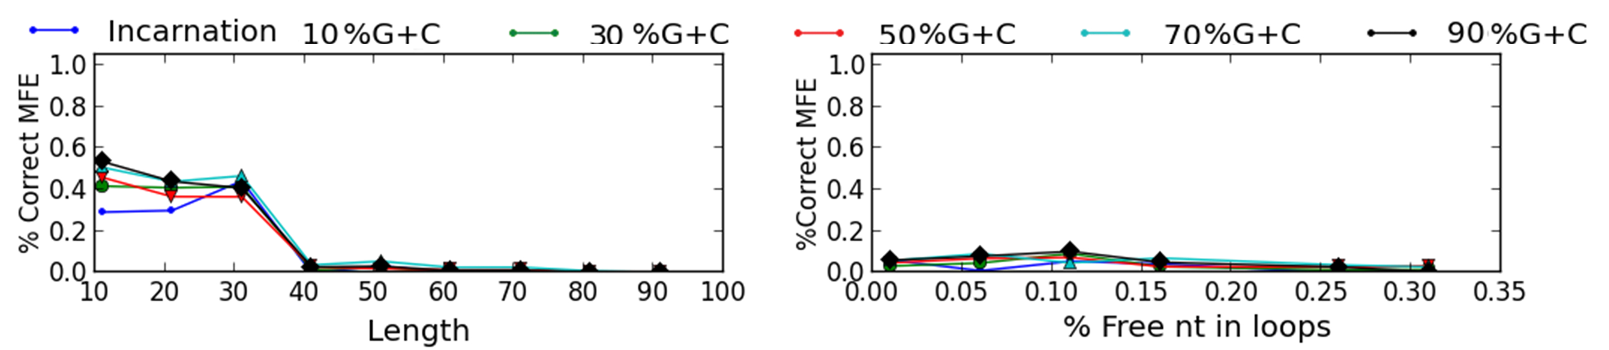
\includegraphics[width=1.1\textwidth]{Figures/results_incar.pdf}
%	\end{figure}
%
%}
%
%\frame{
%	\frametitle{Incarnation + RNAinverse nt distribution}
%	\begin{table}[ht!]
%\begin{center}
%\resizebox{\textwidth}{!}{
%\begin{tabular}{|c|c|c|}
%\hline
%\multirow{3}{*}{Target \GCContent (\%)}& \multicolumn{2}{c|}{\GCContent (\%) of designed sequences}\\ \cline{2-3}
% & \ourprog & \ourprog + \RNAinverse\\
% & (Global) & ({Glocal}) \\
%\hline
%10\% & 15\% & 21\% \quad $\nearrow 6\%$\\
%30\% & 30\% & 33\% \quad $\nearrow 3\%$\\
%50\% & 48\% & 49\% \quad $\nearrow 1\%$\\
%70\% & 71\% & 69\% \quad $\searrow 2\%$\\
%90\% & 83\% & 78\% \quad $\searrow 5\%$\\
%\hline
%\end{tabular}
%}
%\end{center}
%\label{table:impact_on_gc}
%\end{table}
%}
%
%\frame{
%	\frametitle{Incarnation + RNAinverse Results }
%	\begin{figure}[t!]
%		\centering
%		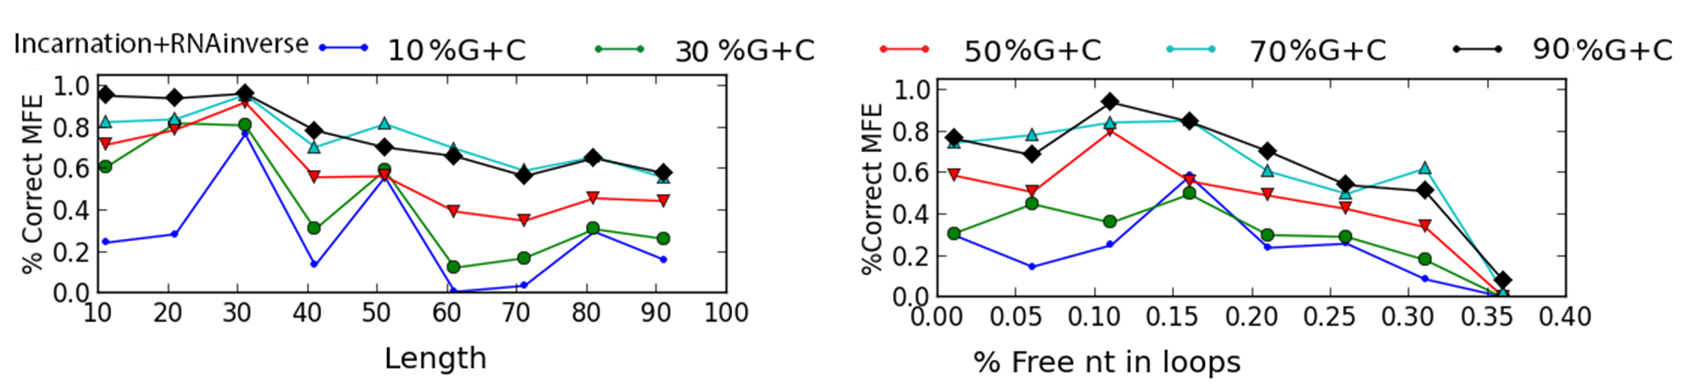
\includegraphics[width=1.1\textwidth]{Figures/results_incar_rnainverse.pdf}
%	\end{figure}
%% 	\pause
%%	\begin{figure}
%%		\centering
%%		\includegraphics[width=1.1\textwidth]{Figures/Sensitivity.pdf}
%%		\caption{Structural sensitivity (\#bp well predicted/\#bp target)}
%%	\end{figure}
%}
%
%\frame{
%	\frametitle{Incarnation + RNAinverse Results\\Sequence identity}
%	\begin{figure}[t!]
%		\centering
%		\includegraphics[width=1.1\textwidth]{Figures/identity.png}
%	\end{figure}
%}
%
%\frame{
%	\frametitle{Incarnation + RNAinverse time}
%	\begin{figure}[t!]
%		\centering
%		\includegraphics[width=0.9\textwidth]{Figures/time.png}
%	\end{figure}
%}
%
%\frame{
%	\frametitle{Future}
%	\begin{itemize}
%		\item Full energy model
%		\item Include other seeded methods
%		\item Convince people to make the molecules in labs
%	\end{itemize}
%}
%
%\frame{
%	\frametitle{Acknowledgments}
%	\begin{minipage}{0.45\textwidth}
%		\begin{itemize}
%			\item Coauthors
%			\begin{itemize}
%				\item \JW
%				\item \YP		
%			\end{itemize}
%		\end{itemize}	
%	\begin{figure}
%		\centering
%		\includegraphics[width=0.5\textwidth]{Figures/logofsm}
%	\end{figure}
%	\end{minipage}
%	\begin{minipage}{0.45\textwidth}
%		\begin{itemize}
%			\item Erasmus TEE  fellowship
%		\end{itemize}
%%			\item  French Agence Nationale de la Recherche (ANR) through the {\sc Magnum} {\tt ANR 2010 BLAN 0204} 
%%project (to YP), 
%%			\item FQRNT team grant 232983 (to VR and JW) 
%%			\item NSERC Discovery grant 219671 (to JW).
%%		\end{itemize}	
%		\begin{minipage}{0.45\textwidth}
%		\begin{figure}
%			\centering
%			\includegraphics[width=\textwidth]{Figures/logoanr.png}
%		\end{figure}
%		\begin{figure}
%				\centering
%			\includegraphics[width=\textwidth]{Figures/logoinria.png}
%		\end{figure}
%		\begin{figure}
%			\centering
%			\includegraphics[width=\textwidth]{Figures/logofqrnt.png}
%		\end{figure}
%		\end{minipage}
%		\begin{minipage}{0.45\textwidth}
%		\begin{figure}
%			\centering
%			\includegraphics[width=\textwidth]{Figures/logonserc}
%		\end{figure}
%		\begin{figure}
%			\centering
%			\includegraphics[width=\textwidth]{Figures/logocnrs}
%		\end{figure}
%		\begin{figure}
%			\centering
%			\includegraphics[width=\textwidth]{Figures/logo_X}
%		\end{figure}
%		\end{minipage}		
%	\end{minipage}
%}
%



%}
%
%\frame{
%	\frametitle{And so...}
%		\begin{itemize}
%			\item It kinda works
%			\item Energetic model really simple
%			\item Exploit sequences with wanted structures (but wrong GC content).
%		\end{itemize}
%	\begin{minipage}{0.45\textwidth}
%		\begin{equation*}
%		\label{eq:Z_rec}
%		\resizebox{\textwidth}{!}{%
%			$\Z{i,j}{m}{a,b}:=\left\{
%	  \begin{array}{ll}
%  		\displaystyle
%      \sum_{\substack{a'\in \B,\\ \Kron_{a',s_i}\le m}}  
%      \Z{i+1,j}{m-\Kron_{a',s_i}}{a',b} & \text{If }S_{i}=-1\\
%      \displaystyle
%      \sum_{\substack{a',b'\in \B^2,\\ \Kron_{a'b',s_is_j}\le m}}
%			 e^{\frac{-E_{(i,j),ab \to a'b'}^{\Omega,\beta}}{RT}}
%			 \cdot \Z{i+1,j-1}{m-\Kron_{a'b',s_is_j}}{a',b'}&
%			 \text{Elif }S_i=j \land S_{i-1}=j+1\\
%			 \displaystyle
%      \sum_{\substack{a',b'\in \B^2,\\ \Kron_{a'b',s_is_k}\le m}}
%      \sum_{m'=0}^{m-\Kron_{a'b',s_is_k}}
%   		 e^{\frac{-E_{(i,k),\varnothing\to a'b'}^{\Omega,\beta}}{RT}}
%      \cdot\Z{i+1,k-1}{m-\Kron_{a'b',s_is_k}-m'}{a',b'}
%      \cdot\Z{k+1,j}{m'}{b',b} & \text{Elif }S_i=k \land i < k \leq j\\
%      0 &\text{Otherwise}
%		\end{array}\right.$}
%		\end{equation*}
%	\end{minipage}
%	\begin{minipage}{0.45\textwidth}
%	\begin{algorithm}
%		bob
%	\end{algorithm}
%	\begin{algorithm}[t]
%		\DontPrintSemicolon
%		\SetAlgoLined
%		\SetKwFunction{Backtrack}{SB$_x$}
%		\SetKwFunction{Random}{Random}
%		\newcommand{\rand}{{r}}
%		$\rand \leftarrow $\Random$\left(\Z{\N,\Struct}{a,b}\right)$\tcp*[r]{Random 		real in $[0,\Z{\N,\Struct}{a,b}[$}
%		 \Switch{}{
%   		\lCase(\tcp*[f]{Empty structure}){$\Struct=\varepsilon$}{\Return{$\varepsilon$}}
%		  \Case(\tcp*[f]{First position is unpaired}){$\Struct=\ub\, \Struct'$}{		
%   			\For{$a'\in\B$}{
%					$\rand \leftarrow \rand - x^{\gc(a')}\cdot \Z{\BoolFalse,\Struct'}{a',b}$\;
%					\lIf{$\rand<0$}\Return{$a'.\Backtrack(a',b,\BoolFalse,\Struct')$}\;
%  			}
%   		}
%	   	\Case(\tcp*[f]{Extremities are involved in stacking base pair}){$\Struct=			\text{\rm\op}\, \Struct' \,\text{\rm\cp}$  {\rm \bf and} $\N=\BoolTrue$}
%   		{		
%				\For{$(a',b')\in\B\times\B$}
%    		{
%					$\rand \leftarrow \rand -
%			 		x^{\gc(a'.b')}
%			 		\cdot e^{{-\ES^{\beta}_{ab \to a'b'}}/{RT}}
%			 		\cdot \Z{\BoolTrue,\Struct'}{a',b'}	$\;
%					\lIf{$\rand<0$}{
%						\Return{$a'.\Backtrack(a',b',\BoolTrue,\Struct'). b'$}\;		
%					}
%				}
%			}
%   		\Other(\tcp*[f]{First position is paired without a stacking pair})
%   		{
%				\tcp{$\Struct=\text{\rm\op}\, \Struct' \,\text{\rm\cp}\,\Struct''$}
%				\For{$(a',b')\in\B\times\B$}{
%					$\rand \leftarrow \rand -	
%    	   	x^{\gc(a'.b')}
%					\cdot e^{\frac{-\ES^{\beta}_{\varnothing\to a'b'}}{RT}}
%	  	    \cdot\Z{\BoolFalse,\Struct'}{a',b'}
%	      	\cdot\Z{\BoolTrue,\Struct''}{b',b}$\;	
% 					\lIf{\rand $<0$}{
%						\Return{$a'
%							.\Backtrack\left(a',b',\BoolTrue,\Struct'\right)
%							.b'
%							.\Backtrack\left(b',b,\BoolFalse,\Struct''\right)
%						$}\;	
%					}
%				}
%   		}
%	 	}
%\caption{\protect\Backtrack$\left(a,b,\N,\Struct\right)$\label{alg:back}}
%\end{algorithm}
%\end{minipage}
%
%}


\end{document}



